\documentclass[a4paper,oneside,12pt]{article}
\usepackage[portuguese]{babel}
\usepackage{graphicx}
\usepackage{listings}
\usepackage{indentfirst}

\usepackage{xcolor}

\definecolor{codegreen}{rgb}{0,0.6,0}
\definecolor{codegray}{rgb}{0.5,0.5,0.5}
\definecolor{codepurple}{rgb}{0.58,0,0.82}
\definecolor{backcolour}{rgb}{0.95,0.95,0.92}

\lstdefinestyle{mystyle}{
    backgroundcolor=\color{backcolour},   
    commentstyle=\color{codegreen},
    keywordstyle=\color{magenta},
    numberstyle=\tiny\color{codegray},
    stringstyle=\color{codepurple},
    basicstyle=\ttfamily\footnotesize,
    breakatwhitespace=false,         
    breaklines=true,                 
    captionpos=b,                    
    keepspaces=true,                 
    numbers=left,                    
    numbersep=5pt,                  
    showspaces=false,                
    showstringspaces=false,
    showtabs=false,                  
    tabsize=2
}

\lstset{style=mystyle}

\linespread{1.5}

\usepackage{fontspec}
\setmainfont{Times New Roman}

\title{Arquivos Binários}
\author{Canoi Gomes}
\date{23 de Junho de 2024}


\begin{document}
\maketitle
\newpage

\tableofcontents
\newpage

\section{Introdução}

Você sabe como funciona um arquivo binário? Aqueles arquivos que ao tentarmos abrir num editor de textos qualquer, aparece um monte de símbolos que mal dá para entender do que se trata. Bem, e se eu te disser que tem uma lógica por trás deles? E isso é mais ou menos o que quero abordar nessas linhas.

\subsection{O que é um arquivo binário?}

Simplificando bastante, um arquivo binário nada mais é que um arquivo de texto, porém formatado de uma maneira bem específica onde o programa que for fazer uso daquele arquivo deve saber como é a sua estrutura interna. Quando digo que não se difere muito do arquivos de texto, é porque temos isso com eles também, se criamos um arquivo JSON ou XML, também temos uma estrutura que se for bagunçada é o suficiente para corromper o arquivo.
Da mesma forma ambos são usados para guardar algum tipo de informação. A principal diferença é que arquivos de texto estão preocupados com os caracteres do arquivo, já um arquivo binário se preocupa com como os bytes estão posicionados, e até mesmo cada bit.

Alguns formatos de arquivos binários que posso citar são o .zip, .bmp, .wav, .png, que como vocês podem ver são usados para guardar diferentes tipos de dados. Até mesmo os nossos arquivos executáveis (PE no Windows (.exe) e ELF no Linux) são binários, e o nosso sistema operacional que sabe como interpretá-los. Mais pra frente quando eu for mostrar a estrutura de alguns formatos mais populares (.bmp, .tar, .wav, ...), você vai ver que é possível até mesmo interpretar o que está dentro de arquivos binários executáveis.

\section{Criando um Formato de Arquivo Binário}

Beleza, mas por onde podemos começar se queremos escrever um formato de arquivo binário e um programa que seja capaz de o interpretar?

Bom, veja esses exemplos:

\noindent
\textbf{file.json}:
\begin{lstlisting}
{
    "magic": "MF",
    "name": "Ze Brasileiro",
    "idade": 25,
    "vivo": true
}
\end{lstlisting}

\noindent
\textbf{file.bin}:
\begin{lstlisting}
MFZe Brasileiro@$
\end{lstlisting}

Coloquei esses símbolos no final só para representar que algo foi escrito naqueles campos, mas imagine que ali o @ representa 25 e \$ representa 1. Mas perceba que ambos guardam o mesmo tipo de informação, dados sobre nome, idade, se a pessoa está viva, e o magic ali é pra representar um \textbf{magic number}, é comum em formatos de arquivos binários você ter um desses, ele serve basicamente para validação do tipo. Por exemplo, caso você crie um programa que vá ler especificamente esse seu formato, então quando um usuário for tentar abrir um arquivo qualquer, você checa se a magic desse arquivo é de fato ``MF'', e caso contrário você retorna uma mensagem de erro dizendo que o tipo é inválido. É um jeito mais seguro que só checar pela extensão do arquivo, por exemplo.

\subsection{Tabela ASCII}

Para entender o que aconteceu com os valores de Idade (25) e Vivo (true, ou 1), precisamos entender como funciona a construção de uma string e o que é uma tabela ASCII.

Vamos analisar nosso arquivo usando um editor hexadecimal:

\begin{figure}[h]
    \centering
    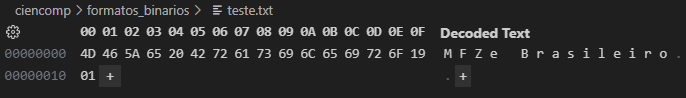
\includegraphics[width=\linewidth]{media/hex.png}
\end{figure}

Perceba como cada caractere tem um valor hexadecimal correspondente. Para entender esses valores você pode conferir a tabela ASCII abaixo.

\begin{figure}[h]
    \centering
    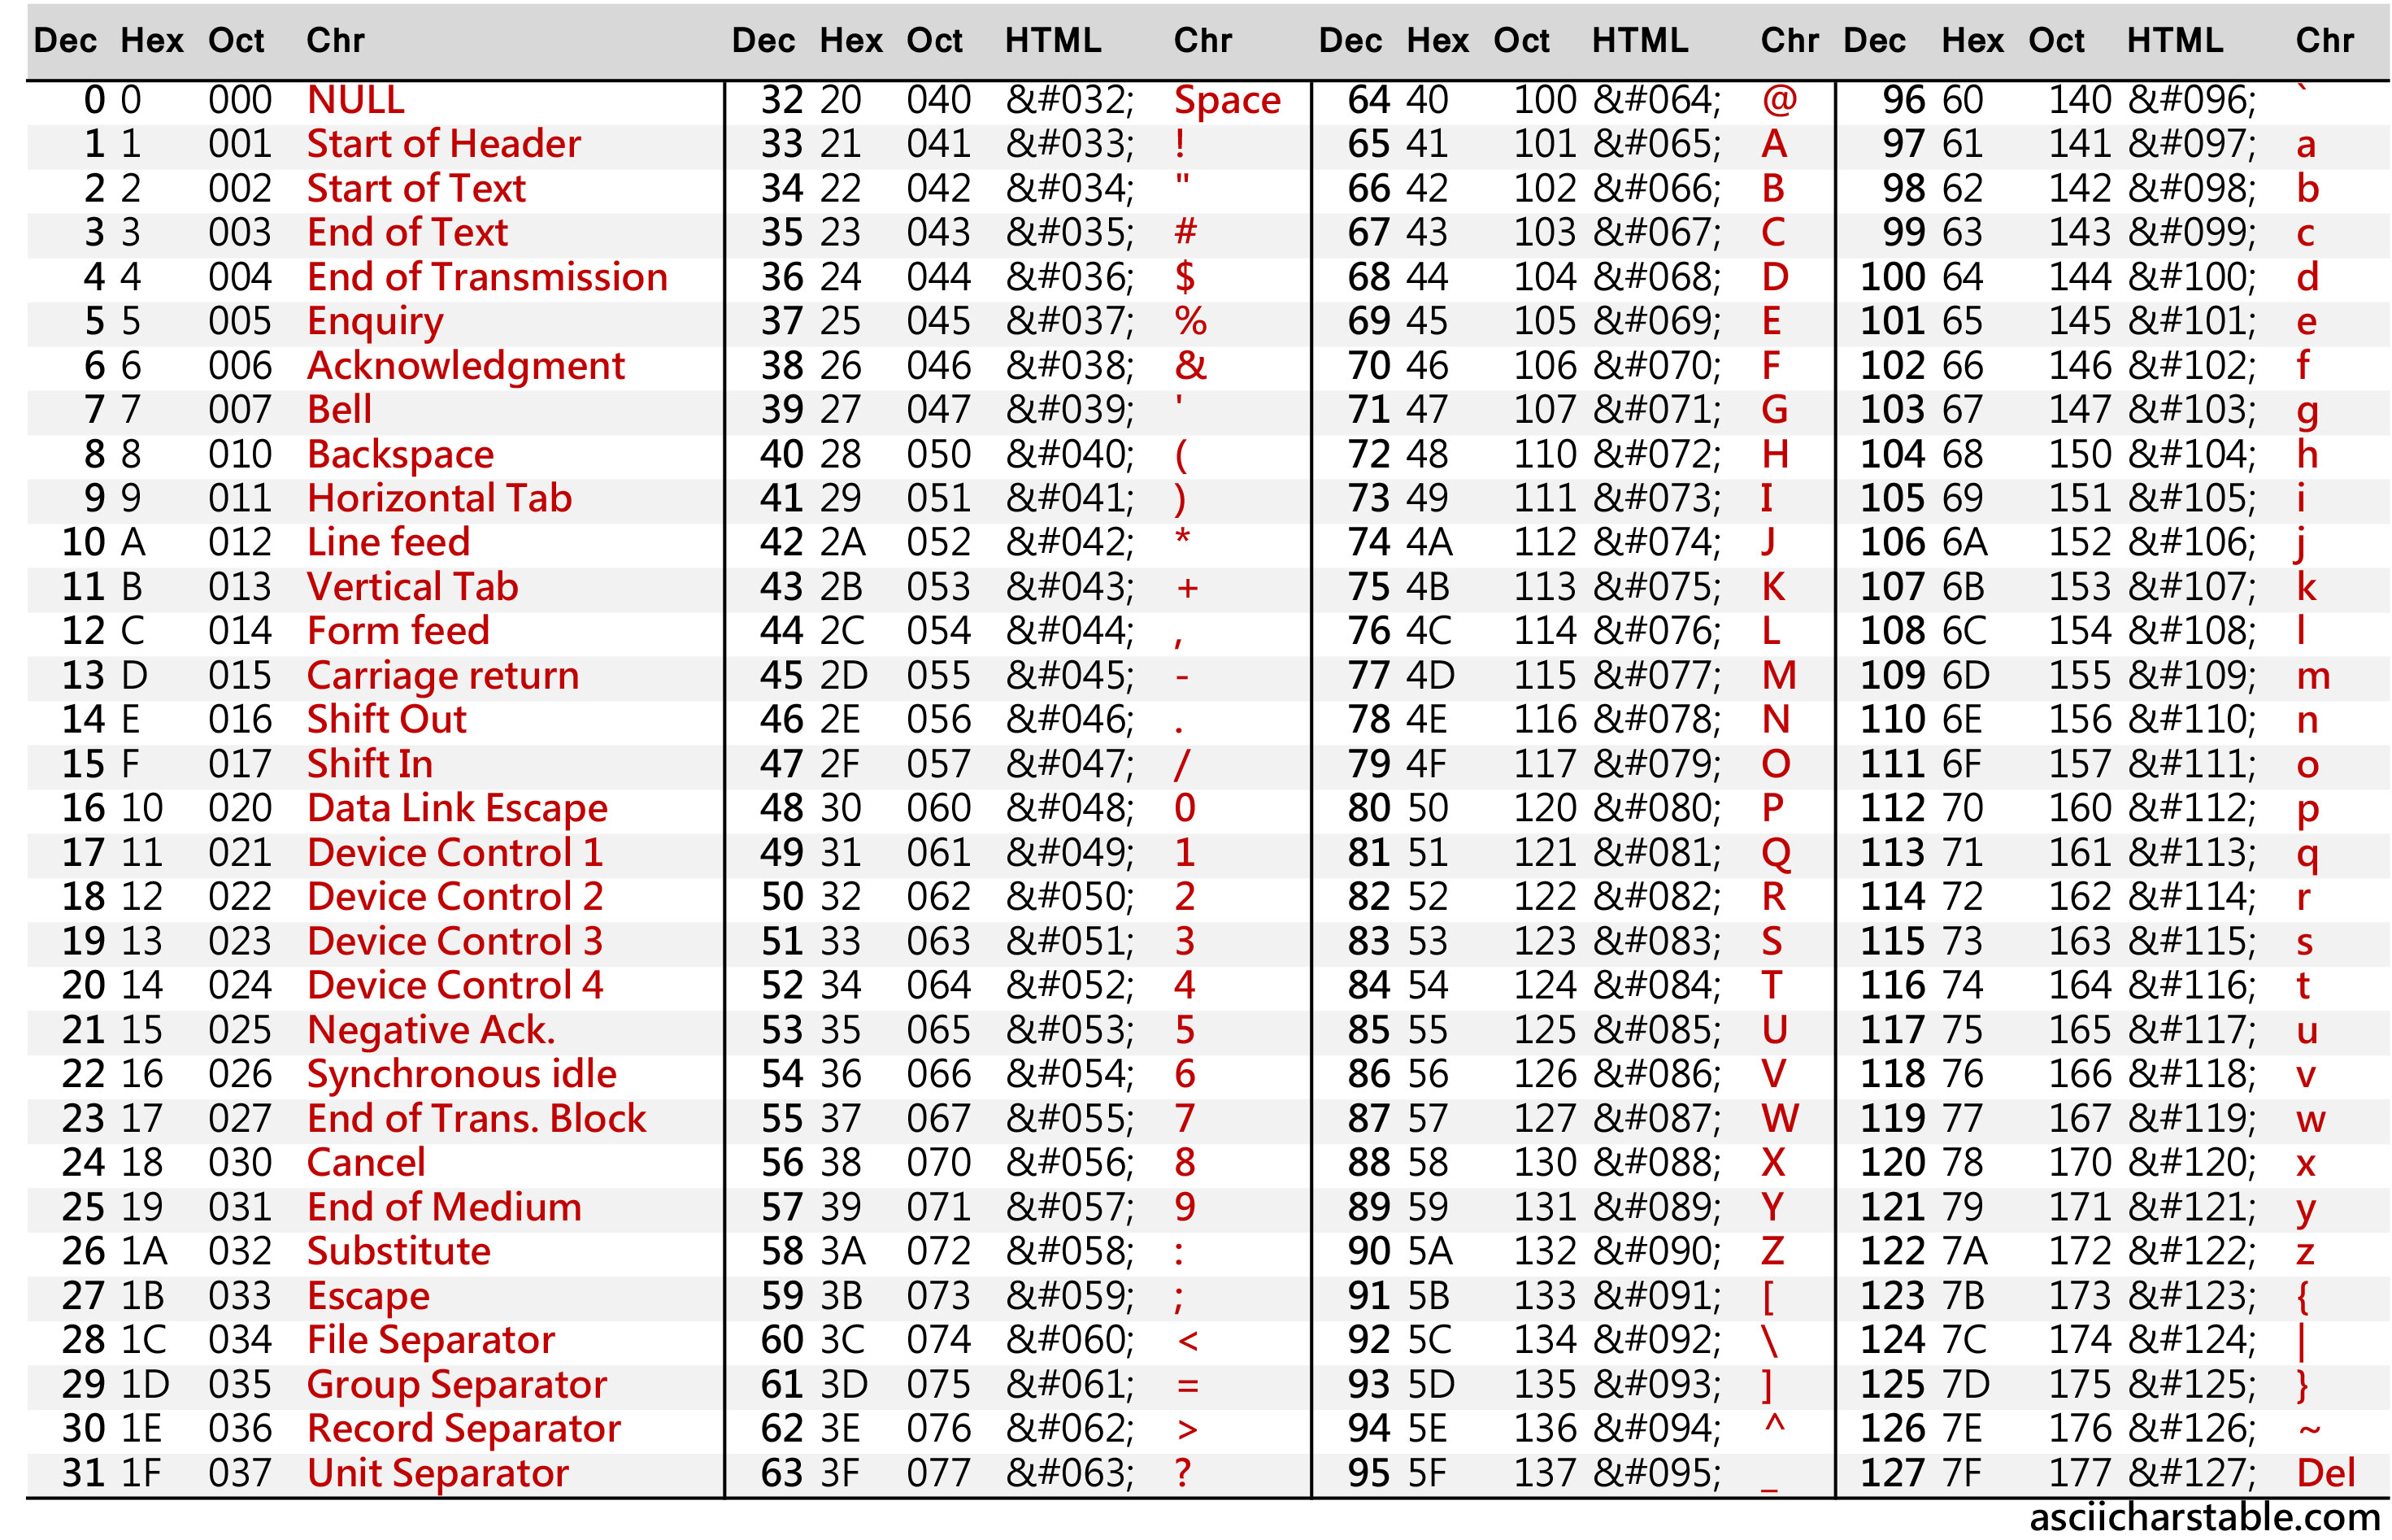
\includegraphics[width=\linewidth]{media/ASCII.jpg}
\end{figure}

Então olhando com mais calma:
\begin{itemize}
    \item 0x4D e 0x46: Representa o nosso magic number, \textbf{4D = M} e \textbf{46 = F}
    \item 0x5A ao 0x6F: Representa o nosso nome, se pegarmos novamente na tabela ASCII vamos ver que \textbf{5A = Z} e \textbf{6F = o}
    \item 0x19 e 0x01: Essa que é a parte interessante, se pegarmos na tabela vamos ver que esses códigos representam caracteres especiais. Caracteres esses que muito provavelmente não serão exibidos no editor de texto. Porém o que nos interessa não é o caractere que o código representa, e sim seu valor. 0x19 é o valor hexadecimal para 25, ou seja, a idade que nós colocamos para a pessoa. Igualmente o 0x01, o que nos interessa é somente o seu valor (true nesse caso).
\end{itemize}

\subsection{Cabeçalho}

Tá bom, mas como que eu represento isso no meu código? É bem comum utilizar algo chamado cabeçalho, que vai ter uma representação exata dos bytes utilizados por cada campo.
Eu vou começar alterando um pouco o formato do meu tipo. No cabeçalho não vou guardar as informações relativas ao nome, e sim qual o tamanho do nome. E o dado do nome de fato, eu escrevo depois do meu cabeçalho. Seria algo mais ou menos assim:
\begin{lstlisting}
MF#@$Ze Brasileiro
\end{lstlisting}
Ignore os simbolos de \textbf{\#, @ e \$} por agora, só saiba que eles representam respectivamente o [tamanho do nome][idade][vivo ou morto].

Representando em uma struct em C eu vou ter isso aqui:
\begin{lstlisting}[language=C, caption=Cabeçalho em C]
struct Header {
    char magic[2];
    char name_size;
    char age;
    char alive;
};
\end{lstlisting}

Mas por que eu fiz isso? Bem, como estava anteriormente, com o nome vindo logo depois do magic number, um trabalho a mais é necessário para se interpretar esse arquivo. Seria necessário ler inicialmente os dois bytes, e depois começar a ler caractere por caractere do nome até chegar em um número. Com isso eu não consigo identificar facilmente o tamanho do nome de cara, preciso fazer essa leitura byte a byte e pode dificultar um pouco no uso no programa.

Uma convenção bem comum é setar um tamanho fixo de bytes para guardar uma string.

\begin{lstlisting}[language=C, caption=Cabeçalho com tamanho fixo de string]
struct Header {
    char magic[2];
    char name[32];
    char age;
    char alive;
};
\end{lstlisting}

Ou seja, seu nome não pode ser maior que 32 bytes, porém pode ser menor. Só que nesse caso, mesmo que o nome seja menor que 32 bytes, a informação da idade não vem logo depois do nome, ela começa somente no byte 34 (2 do magic + 32 do nome), pois o resto dos bytes será preenchido (provavelmente com 0). Teria algo assim:

\begin{lstlisting}
MFZe Brasileiro0000000000000000000@$
\end{lstlisting}

Novamente, isso é só uma representação, é muito provável que no seu editor de textos você não veja nenhum símbolo após o nome.

\subsection{Escrevendo em um arquivo binário}

Mas vamos para o código em C.

\begin{lstlisting}[language=C, caption=Exemplo de escrita em C]
#include <stdio.>
#include <string.h>

struct Header {
    char magic[2]; // magic number "MF"
    char name_size; // quantidade de bytes que tem meu nome
    char age; // idade
    char alive; // vivo (1 para true, 0 para false)
};

int main(int argc, char** argv) {
    FILE* fp = fopen("file.bin", "wb"); // abrindo o arquivo file.bin em modo de escrita binária
    const char* name = "Ze Brasileiro";
    struct Header h;
    h.magic[0] = 'M';
    h.magic[1] = 'F';
    h.name_size = strlen(name); // pego tamanho do nome em bytes
    h.age = 25;
    h.alive = 1;
    fwrite(&h, 1, sizeof(h), fp); // escrevo o cabeçalho no inicio do arquivo
    fwrite(name, 1, h.name_size, fp); // escrevo o nome logo em seguida
    fclose(fp);
    return 0;
}
\end{lstlisting}

Aqui não tem muito mistério. Eu preencho meu cabeçalho com os dados que quero utilizar e escrevo em um arquivo (lembre-se de abrir o arquivo no modo de escrita binária, ou \textbf{wb}), e logo em seguida escrevo o nome.

\subsection{Lendo de um arquivo binário}

Bom, e caso eu queira ler esse arquivo que eu acabei de criar. Continua sendo bem simples, a gente só precisar usar o mesmo cabeçalho, e dessa vez ao invés de abrir o arquivo no modo de escrita binária (\textbf{wb}), irei abrir no modo de leitura binária (\textbf{rb}):

\begin{lstlisting}[language=C, caption=Exemplo de leitura em C]
#include <stdio.>
#include <string.h>

struct Header {
    char magic[2]; // magic number "MF"
    char name_size; // quantidade de bytes que tem meu nome
    char age; // idade
    char alive; // vivo (1 para true, 0 para false)
};

int main(int argc, char** argv) {
    FILE* fp = fopen("file.bin", "rb"); // abrindo o arquivo file.bin em modo de leitura binária
    struct Header h;
    fread(&h, 1, sizeof(h), fp); // leio o cabeçalho no inicio do meu arquivo
    if (h.magic[0] != 'M' || h.magic[1] != 'F') return -1; // formato inválido
    char name[h.name_size+1];
    fread(name, 1, h.name_size, fp); // em seguida leio [name_size] bytes, que é o tamanho do meu nome
    name[h.name_size] = '\0';

    printf("nome: %s\n", name);
    fclose(fp);
    return 0;
}
\end{lstlisting}

\subsection{Formato Binário Legível}

Só para finalizar o assunto, também é possível construirmos um formato binário que seja legível/modificável por um editor de textos comum. Você só tem que se atentar com a maneira que seu programa interpreta o arquivo. Se eu quiser fazer algo assim, por exemplo:

\begin{lstlisting}
MF13251Ze Brasileiro
\end{lstlisting}

É preciso notar que cada um dos números representam um caractere a parte. Ou seja, o 13 nós precisamos tratar como 1 e 3 tendo bytes separados, a mesma coisa pro 25. Poderia fazer um cabeçalho assim, por exemplo:

\begin{lstlisting}[language=C]
struct Header {
    char magic[2];
    char name_size[2];
    char age[2];
    char alive;
};
\end{lstlisting}

Mas para usar os valores reais é preciso converter de string para número:

\begin{lstlisting}
13
1 (0x49 em ASCII) e 3 (0x51 em ASCII)
value = (1 - 0x48) * 10 + (3 - 0x48);
\end{lstlisting}

\section{Considerações}

Acho que é isso que tinha para escrever por agora, é só uma pincelada no assunto para entender como funciona a estrutura de um arquivo binário. Como falei anteriormente, nos próximos textos vai ficar mais fácil de entender isso quando estivermos lidando com formatos de arquivo binário mais consolidados.

\end{document}